\documentclass[11pt,letterpaper,notitlepage]{article}

%================== Document nomenclature
\newcommand{\DOCSUBJT}{Whitepaper: }   %Put document subject here
\newcommand{\DOCTITLE}{                      %Put document title here
 K-Eigenvalue solver schemes in LBS
}       
\newcommand{\DOCDATE} {April, 2023}         %Put document date here
\newcommand{\DOCREV}  {Rev 1.00}             %Put revision number here

%================== Misc Settings
\usepackage{fancyhdr}
\usepackage[left=0.75in, right=0.75in, bottom=1.0in]{geometry}
\usepackage{lastpage}
\usepackage{titleref}
\usepackage{booktabs}
\usepackage{appendix}

\appendixtitleon
\appendixtitletocon

\makeatletter

%================== RangeList of figures and tables mods
\usepackage{tocloft}
\usepackage[labelfont=bf]{caption}

\renewcommand{\cftfigpresnum}{Figure\ }
\renewcommand{\cfttabpresnum}{Table\ }

\newlength{\mylenf}
\settowidth{\mylenf}{\cftfigpresnum}
\setlength{\cftfignumwidth}{\dimexpr\mylenf+3.5em}
\setlength{\cfttabnumwidth}{\dimexpr\mylenf+1.5em}
\renewcommand{\cftsecdotsep}{\cftdotsep} % dotted chapter leaders

\usepackage{bookmark}
\hypersetup{	pdfborder = {0 0 0} }
\setcounter{tocdepth}{5}
\setcounter{secnumdepth}{5}


%=================== Misc packages
\usepackage{graphicx}
\usepackage[breakwords]{truncate}
\usepackage{float}
\usepackage{array}
\usepackage{amsmath}
\usepackage{mdframed}
\usepackage{fancyvrb}
\usepackage{float}
\usepackage{cancel}
\usepackage{amssymb}
\graphicspath{ {images/} }
\usepackage[usenames,dvipsnames,svgnames,table]{xcolor}
%\usepackage[defaultlines=2,all]{nowidow}
\usepackage{listings}
\usepackage{color}
\definecolor{Brown}{cmyk}{0,0.81,1,0.60}
\definecolor{OliveGreen}{cmyk}{0.64,0,0.95,0.40}
\definecolor{CadetBlue}{cmyk}{0.62,0.57,0.23,0}
\usepackage{pdflscape}
\usepackage{relsize}
\usepackage{verbatim}
\usepackage{tabto}
%\usepackage{upgreek}
\usepackage{enumitem}
%\usepackage{MnSymbol}% http://ctan.org/pkg/mnsymbol
\usepackage[pdf]{graphviz}
\usepackage[linesnumbered,lined,boxruled,algosection,commentsnumbered]{algorithm2e}
\usepackage{enumitem}
\usepackage{multicol}
\usepackage{lipsum} %Bunch of garbage paragraphs for testing

\definecolor{gray}{rgb}{0.4,0.4,0.4}
\definecolor{darkblue}{rgb}{0.0,0.0,0.6}
\definecolor{cyan}{rgb}{0.0,0.6,0.6}

\definecolor{ao(english)}{rgb}{0.0, 0.5, 0.0}

\newcommand{\xmltag}[1]{\textcolor{blue}{ \texttt{#1}} }
\newcommand{\xmloption}[1]{\textcolor{ao(english)}{ \texttt{#1}} }


\counterwithin{figure}{section}
\renewcommand{\thefigure}{\arabic{section}.\arabic{figure}}


\newcommand{\beq}{\begin{equation*}
		\begin{aligned}}
		\newcommand{\eeq}{\end{aligned}
\end{equation*}}

\newcommand{\beqn}{\begin{equation}
		\begin{aligned}}
		\newcommand{\eeqn}{\end{aligned}
\end{equation}}

%=================== Settings
\renewcommand{\baselinestretch}{1.2}
\definecolor{gray}{rgb}{0.4 0.4 0.4}
\newcommand{\stimes}{{\times}}

%================== Code syntax highlighting
\lstset{language=C++,frame=ltrb,framesep=2pt,basicstyle=\linespread{0.8} \small,
	keywordstyle=\ttfamily\color{OliveGreen},
	identifierstyle=\ttfamily\color{CadetBlue}\bfseries,
	commentstyle=\color{Brown},
	stringstyle=\ttfamily,
	showstringspaces=true,
	tabsize=2,}

%================== Section numbers with equation numbers
\numberwithin{equation}{section}


%================== Short \to arrow
\setlength{\medmuskip}{0mu}
%\newcommand{\tos}[1][3pt]{\mathrel{%
		%   \hbox{\rule[\dimexpr\fontdimen22\textfont2-.2pt\relax]{#1}{.4pt}}%
		%   \mkern-4mu\hbox{\usefont{U}{lasy}{m}{n}\symbol{41}}}}



%\setlength\parindent{0pt}

%
% Bold quantities
% 
\newcommand{\Omegabf}{\mathbf{\Omega}}
\newcommand{\bnabla}{\boldsymbol{\nabla}}
\newcommand{\position}{\mathbf{x}}
\newcommand{\dotp}{\boldsymbol{\cdot}}

\newcommand{\Linv}{L^{-1}}
\newcommand{\bphi}{\boldsymbol{\phi}}
\newcommand{\bpsi}{\boldsymbol{\psi}}
\newcommand{\br}{\mathbf{r}}
\newcommand{\bR}{\mathbf{R}}
\newcommand{\half}{\frac{1}{2}}
\newcommand{\bepsilon}{\boldsymbol{\epsilon}}
%
% Vector forms
%
\renewcommand{\vec}[1]{\mbox{$\stackrel{\longrightarrow}{#1}$}}
\renewcommand{\div}{\mbox{$\vec{\mathbf{\nabla}} \cdot$}}
\newcommand{\grad}{\mbox{$\vec{\mathbf{\nabla}}$}}
\newcommand{\bb}[1]{\bar{\bar{#1}}}
%
% Vector forms boldfaced
\newcommand{\bvec}[1]{\mathbf{#1}}
\newcommand{\bdiv}{\boldsymbol{\nabla} \boldsymbol{\cdot}}
\newcommand{\bgrad}{\bnabla}
\newcommand{\mat}[1]{\bar{\bar{#1}}}


% Background pic
% Use	\AddToShipoutPicture*{\BackgroundPic} for only current page
% and 	\AddToShipoutPicture{\BackgroundPic} for all pages
%
\usepackage{eso-pic}
\newcommand\BackgroundPic{%
	\put(0,0){%
		\parbox[b][\paperheight]{\paperwidth}{%
			\vfill
			\centering
			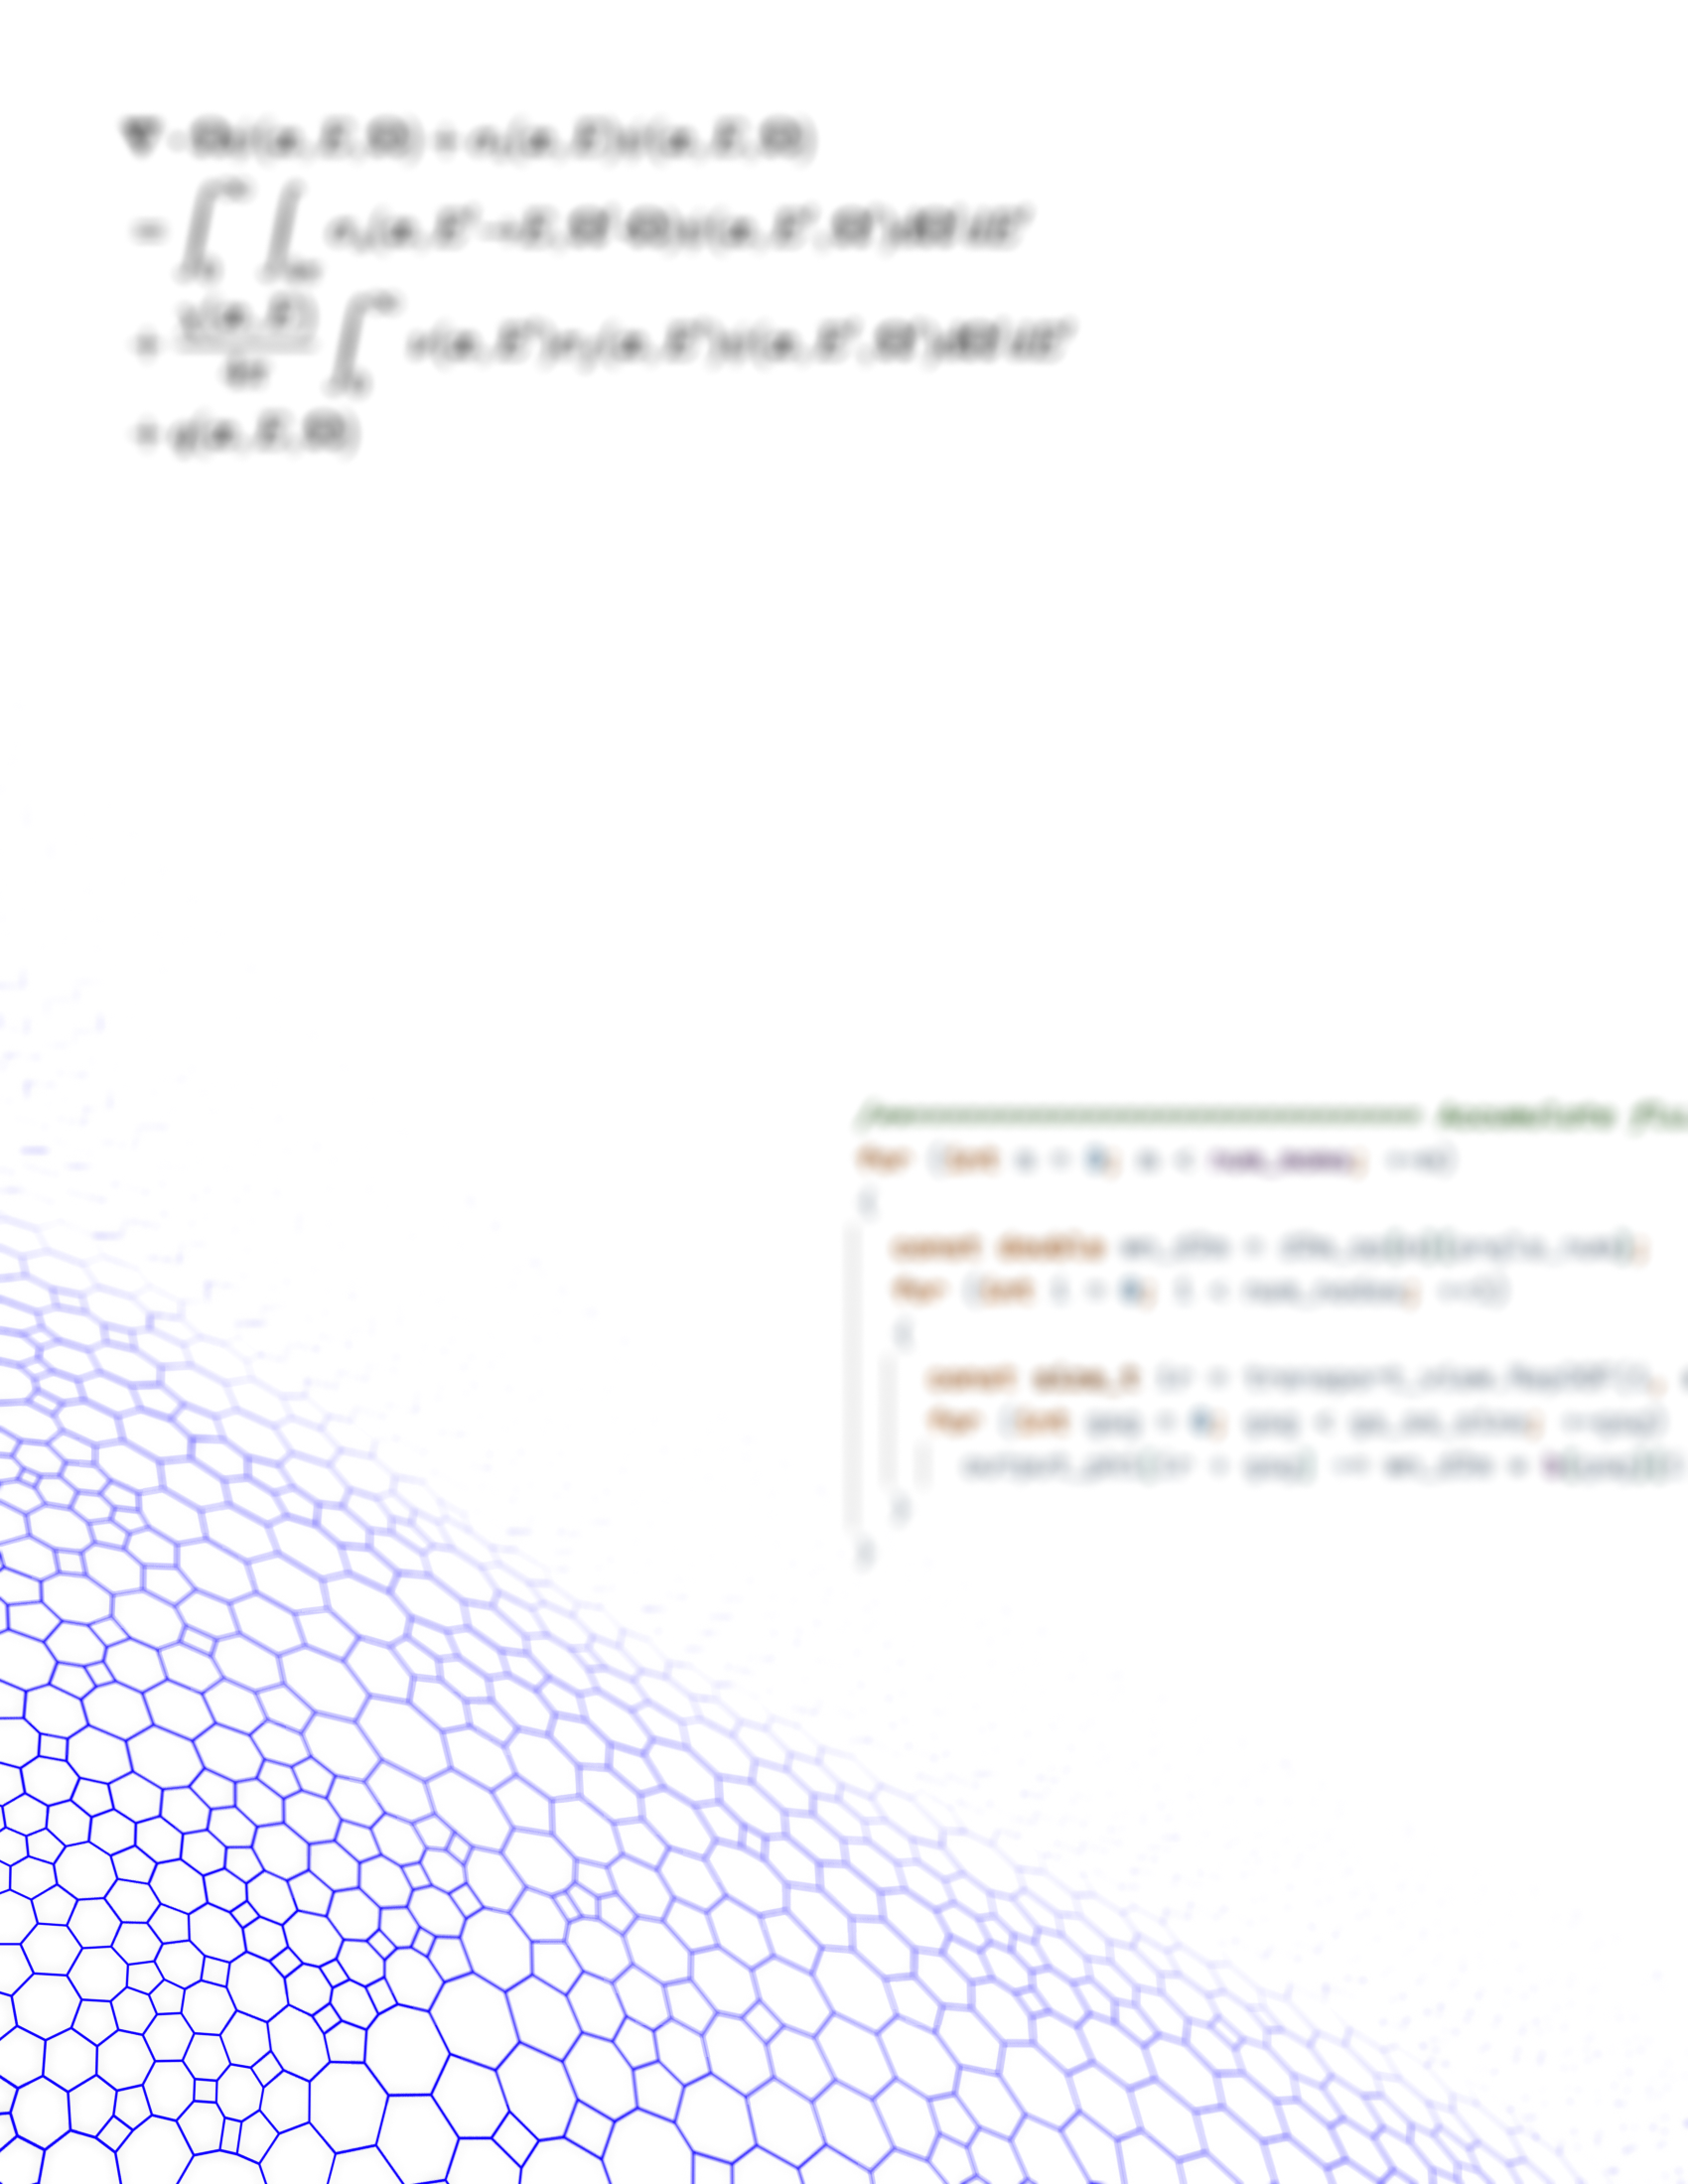
\includegraphics[width=\paperwidth,height=\paperheight,%
			keepaspectratio]{WhitepageBackground.png}%
			\vfill
}}}

%
% Command to make a link back to TOC
%
\newcommand{\BackToTOC}{\hyperlink{toc}{\scriptsize{\color{blue}Back to TOC}}\newline}


\begin{document}
	
\begin{titlepage}
	\AddToShipoutPicture*{\BackgroundPic}
%	\begin{center}
	{\centering 
		\vspace*{3cm}
		{\LARGE\textbf{\DOCSUBJT}}
		
		{\LARGE\textbf{\DOCTITLE}}
		
		\vspace{1cm}
		{\Large \DOCDATE \ \ \DOCREV}
		
		\vspace{1cm}
		{\Large Jan I.C. Vermaak${^{1,2}}$}
		
		\vspace{0.25cm}
		\noindent\rule{\textwidth}{1pt}
		{\small $^1$Idaho National Laboratory, Idaho Falls, Idaho, USA.}
		{\small $^2$Center for Large Scale Scientific Simulations, Texas A\&M Engineering Experiment Station, College Station, Texas, USA.}
		

%	\end{center}



}
\end{titlepage}

\pagestyle{plain}
%\rfoot{Page \thepage \ of \pageref{LastPage}}
\cfoot{\thepage}
%\lfoot{}
%\rhead{}
%\chead{\currentname}
%\lhead{}
%\renewcommand{\footrulewidth}{0.4pt}
%\setlength{\headheight}{13.59999pt}

\pagenumbering{roman}
\chead{Abstract}
\section*{Abstract}\label{abstract}
\addcontentsline{toc}{section}{\nameref{abstract}}


Work is work for some, but for some it is play.
\newline
\newline\noindent
\textbf{Keywords:} transport sweeps; discrete-ordinate method; radiation transport; massively parallel simulations; discontinuous Galerkin; unstructured mesh

\newpage

\chead{Table of contents}

\tableofcontents
\addtocontents{toc}{~\hfill\textbf{Page}\par \protect\hypertarget{toc}{}}

%
\listoffigures
%%\listoftables





\newpage

\pagestyle{fancy}
\rfoot{Page \thepage \ of \pageref{LastPage}}
\cfoot{}
\lfoot{\truncate{14cm}{\DOCTITLE}}
\rhead{}
\chead{\currentname}
\lhead{}
\renewcommand{\footrulewidth}{0.4pt}
\setlength{\headheight}{13.59999pt}

\pagenumbering{arabic}
%\setcounter{secnumdepth}{3}

\chead{Power Iteration}
\section{Power Iteration}\BackToTOC
We start with our discretized transport formulation
\beqn 
(L - MSD)\bpsi = \frac{1}{k} MFD\bpsi
\eeqn 
where
\beqn 
k = ||FD\bpsi ||_2.
\eeqn 

At initialization we assume some shape to the angular flux, e.g. $\psi^\ell=1$ for $\ell=1$. Thereafter we have
\beqn 
(L - MSD)\bpsi^{\ell+1} = \frac{1}{k} MFD\bpsi^{\ell}
\eeqn 
where the right-handside is known, therefore, we solve this equation with our standard steady state tools, i.e. Richardson iteration or GMRes. The term $ \frac{1}{k} FD\bpsi^{\ell}$ is treated as a moment-based source.

\subsection{Inner convergence schemes}\BackToTOC

\subsubsection{Richardson iteration (Source Iteration)}
For richardson iteration we have
\beqn 
L\bpsi^{\ell+1,i+1} &= MSD\bpsi^{\ell+1,i} +  \frac{1}{k^\ell} MFD\bpsi^{\ell} \\
\therefore
\bpsi^{\ell+1,i+1} &= \Linv (MSD\bpsi^{\ell+1,i} +  \frac{1}{k^\ell} MFD\bpsi^{\ell}),
\eeqn 
where $\bpsi^{\ell+1,0} = \bpsi^\ell$.


For a flux-moments based scheme this would be
\beqn 
L\bpsi^{\ell+1,i+1} &= MS\bphi^{\ell+1,i} +  \frac{1}{k^\ell} MF\bphi^{\ell} \\
\therefore 
\bphi^{\ell+1,i+1} &= D\Linv (MS\bphi^{\ell+1,i} +  \frac{1}{k^\ell} MF\bphi^{\ell})
\eeqn 

\subsubsection{Krylov subspace scheme}
For a Krylov subspace scheme we have
\beqn 
L\bpsi^{\ell+1} - MSD\bpsi^{\ell+1} &=  \frac{1}{k^\ell} MFD\bpsi^{\ell}
\eeqn 
which we modify by applying the inverse of the transport operator, $\Linv$, to get
\beqn 
(\Linv \to) \quad \quad 
\bpsi^{\ell+1} - \Linv MSD\bpsi^{\ell+1} &=  \Linv \frac{1}{k^\ell} MFD\bpsi^{\ell} \\
(D \to) \quad \quad 
D\bpsi^{\ell+1} - D\Linv MSD\bpsi^{\ell+1} &=  D\Linv \frac{1}{k^\ell} MFD\bpsi^{\ell}\\
\therefore
\bphi^{\ell+1} - D\Linv MS\bphi^{\ell+1} &=  D\Linv \frac{1}{k^\ell} MF\bphi^{\ell}\\
(I - D\Linv MS) \bphi^{\ell+1} &= D\Linv \frac{1}{k^\ell} MF\bphi^{\ell}
\eeqn 
which can be written in the form
\beqn 
A \bphi^{\ell+1} &= b \\
\eeqn 
where
\beqn
A & = (I - D\Linv MS) \\
\mathbf{b} &= D\Linv \frac{1}{k^\ell} MF\bphi^{\ell}
\eeqn 
and can be solved by a matrix-free Krylov subspace solver e.g. GMRes or BiCGStab.

\subsection{Source Correctred Diffusion Synthetic Acceleration (SCDSA) scheme}
\BackToTOC
\subsubsection{Additive correction formulation}
Suppose we have an unconverged inner result, for which
\beqn 
L\bpsi^{\ell+\half,i} \ne
MS\bphi^{\ell+\half, i} + \frac{1}{k^\ell}MF\bphi^\ell.
\eeqn 
By performing an additional sweep we can get a single update, $\bphi^{\ell+\half,i+1}$, from
\beqn 
\bpsi^{\ell+\half,i+1} = \Linv \biggr(
MS\bphi^{\ell+\half, i} + \frac{1}{k^\ell}MF\bphi^\ell
\biggr)
\eeqn 
allowing us to define the residual of the transport equation, for the update, as 
\beqn
\mathbf{R}^{\ell+\half} = MS\bphi^{\ell+\half,i+1} + \frac{1}{k^\ell}MF\bphi^\ell - L \bpsi^{\ell+\half,i+1}
\eeqn 
but if we plug in the expression for $\bpsi^{\ell+\half,i+1}$ we get
\beqn 
\mathbf{R}^{\ell+\half} = MS\bphi^{\ell+\half,i+1} - MS\bphi^{\ell+\half,i}
\eeqn 
\newline 
Now, the following holds
\beqn 
L \bpsi^{\ell+\half,i+1} - MS\bphi^{\ell+\half,i+1} = \frac{1}{k^\ell} MF\bphi^\ell - \mathbf{R}^{\ell+\half}.
\eeqn 
But we seek
\beqn 
L \bpsi - MS\bphi = \frac{1}{\lambda} MF\bphi
\eeqn 
therefore we subtract these equations
\beqn \label{eq:SCDSA-additive-subtracted}
L(\bpsi-\bpsi^{\ell+\half,i+1}) -MS(\bphi - \bphi^{\ell+\half,i+1})= \frac{1}{\lambda} MF\bphi - \frac{1}{k^\ell} MF\bphi^\ell + \mathbf{R}^{\ell + \half}
\eeqn
and define $\delta \bpsi = \bpsi - \bpsi^{\ell+\half,i+1}$ and $\delta \bphi = \bphi - \bphi^{\ell+\half,i+1}$, the latter from which we rearrange to get $\bphi = \delta \bphi + \bphi^{\ell+\half,i+1}$, allowing us to write 
\beqn 
L\delta \bpsi - MS\delta \bphi &= \frac{1}{\lambda}MF(\delta \bphi + \bphi^{\ell+\half,i+1})  - \frac{1}{k^\ell} MF\bphi^\ell + \mathbf{R}^{\ell + \half}.
\eeqn 
We can now insert our expression for $\mathbf{R}^{\ell + \half}$ to get
\beqn 
L\delta \bpsi - MS\delta \bphi &= \frac{1}{\lambda}MF(\delta \bphi + \bphi^{\ell+\half,i+1})  - \frac{1}{k^\ell} MF\bphi^\ell + MS(\bphi^{\ell+\half,i+1} - \bphi^{\ell+\half,i}),
\eeqn
which takes the form of a k-eigenvalue problem with a source. The diffusion approximation can be applied to this, resulting in
\beqn 
\mathcal{D} \bepsilon - S_{0\mathcal{D}} \bepsilon = \frac{1}{\lambda}F(\bepsilon + \bphi_0^{\ell+\half,i+1}) - \frac{1}{k^\ell} F\bphi_0^\ell + S_0(\bphi_0^{\ell+\half,i+1} - \bphi_0^{\ell+\half,i})
\eeqn 
where $\bepsilon$ are the scalar moments of $\delta \bphi$, $\bphi$ are the scalar moments of $\bphi$, $S_0$ is essentially the same as $S$ except that only the zeroth-moment is non-zero, $S_{0\mathcal{D}}$ is the same as $S_0$ except for the suppression of within-group scattering.


We can solve the above equation using power iteration if we define it as
\beqn 
\mathcal{D} \bepsilon^{k+1} &= S_{0\mathcal{D}} \bepsilon^k + \frac{1}{\lambda^k}F(\bepsilon^k + \bphi_0^{\ell+\half,i+1}) - \frac{1}{k^\ell} F\bphi_0^\ell + S_0(\bphi_0^{\ell+\half,i+1} - \bphi_0^{\ell+\half,i}) \\
&= S_s + S_{f,aux} - S_f + S_{s,\mathbf{R}}
\eeqn 
where $\bepsilon^0 = 0$ and $\lambda^0 = k^\ell$.


\newpage 
\subsubsection{Direct formulation}
For this formulation we start with equation \eqref{eq:SCDSA-additive-subtracted}
\beqn 
L(\bpsi-\bpsi^{\ell+\half,i+1}) -MS(\bphi - \bphi^{\ell+\half,i+1})= \frac{1}{\lambda} MF\bphi - \frac{1}{k^\ell} MF\bphi^\ell + \mathbf{R}^{\ell + \half}
\eeqn
where we mark the supposed analytical solution as the flux at the new iterate $\ell+1$, from which we get
\beqn 
L\bpsi^{\ell+1} &= MS\bphi^{\ell+1} + \frac{1}{k^{\ell+1}}MF\bphi^{\ell+1} \\
&- (MS\bphi^{\ell+\half,i+1} + \frac{1}{k^\ell} MF\bphi^\ell - L\bpsi^{\ell+\half,i+1}) \\
&+ MS\bphi^{\ell+\half,i+1} - MS\bphi^{\ell+\half,i} 
\\
\therefore
L\bpsi^{\ell+1} 
&= MS\bphi^{\ell+1} + \frac{1}{k^{\ell+1}}MF\bphi^{\ell+1} \\
&-(MS\bphi^{\ell+\half,i} + \frac{1}{k^\ell} MF\bphi^\ell - L\bpsi^{\ell+\half,i+1}) \
\eeqn
In this form the subtracted piece at the end of the equation is exactly zero, however, let us first apply the diffusion


\newpage
\chead{Angular flux based non-linear eigenvalue formulation}
\section{Angular flux based non-linear eigenvalue formulation}
\BackToTOC
We start with our discretized transport formulation
\beqn 
(L - MSD)\bpsi = \frac{1}{k} FD\bpsi
\eeqn 
where
\beqn 
k = ||FD\bpsi ||_2
\eeqn 
for which the residual, $\bR$, is given by
\beqn 
\bR(\bpsi) = \frac{1}{k} FD\bpsi - (L - MSD)\bpsi.
\eeqn 
The solution $\bpsi$ approximating a zero residual is then obtained using newton iterations:
\beqn 
\bpsi^{\ell+1} = \bpsi^\ell + \delta \bpsi^\ell
\eeqn 
where
\beqn 
\delta \bpsi^\ell = -J^{-1}(\bpsi^\ell) \bR(\bpsi^\ell)
\eeqn 
obtained from solving the system
\beqn 
J(\bpsi^{\ell}) \delta \bpsi^{\ell} = -\bR(\bpsi^{\ell}).
\eeqn 

This system can be solved using a suitable Krylov Subspace solver (e.g. GMRes), for which we need to still resolve the matrix action $J(\bpsi^{\ell})\mathbf{v}$. For this we use the Jacobian-Free method, involving the approximation 
\beqn 
J(\bphi^{\ell})\mathbf{v} \approx \frac{1}{\epsilon} \biggr(\bR(\bpsi^\ell + \epsilon \mathbf{v}) - \bR(\bpsi^\ell)\biggr)
\eeqn 
where, at each iteration, we need to evaluate $\bR(\bpsi^\ell + \epsilon \mathbf{v})$. Therefore, we define $\bpsi_\epsilon^\ell = \bpsi^\ell + \epsilon \mathbf{v}$ after which we have
\beqn 
\bR(\bpsi^\ell + \epsilon \mathbf{v}) = \bR(\bpsi_\epsilon^\ell).
\eeqn 
\newline
\newline
The linear system can be preconditioned, using the inverse of the transport operator, as
\beqn 
\Linv J(\bpsi^{\ell}) \Delta \bpsi^{\ell} = -\Linv \bR(\bpsi^{\ell}),
\eeqn 
for which all the $\Linv \bR$ terms evaluate to
\beqn
\Linv \bR(\bpsi) &= \frac{1}{k} \Linv FD\bpsi - \bpsi + \Linv MSD\bpsi \\
&= \Delta \bpsi - \bpsi
\eeqn 
where $\Delta \psi$ is obtained by solving the system,
\beqn 
L\Delta \bpsi = \frac{1}{k} FD\bpsi + MSD\bpsi.
\eeqn 

\newpage
\chead{Flux-moments based non-linear eigenvalue formulation}
\section{Flux-moments based non-linear eigenvalue formulation}
\BackToTOC
We start with our flux-moments formulation of the transport system:
\beqn 
(I-D\Linv MS) \bphi = \frac{1}{k} D\Linv F\bphi
\eeqn 
where 
\beqn 
k = ||F\bphi ||_2
\eeqn 
for which the residual, $\br$, is given by
\beqn 
\br(\bphi) = \frac{1}{k} D\Linv F\bphi - (I-D\Linv MS) \bphi.
\eeqn 
The solution $\bphi$ approximating a zero residual is then obtained using newton iterations:
\beqn 
\bphi^{\ell+1} = \bphi^{\ell}  + \delta \bphi^{\ell}
\eeqn
where
\beqn
\delta \bphi^{\ell} = - J^{-1}(\bphi^{\ell}) \br(\bphi^{\ell})
\eeqn 
obtained from solving the system
\beqn 
J(\bphi^{\ell}) \delta \bphi^{\ell} = -\br(\bphi^{\ell}).
\eeqn 

This system can be solved using a suitable Krylov Subspace solver (e.g. GMRes), for which we need to still resolve the matrix action $J(\bphi^{\ell})\mathbf{v}$. For this we use the Jacobian-Free method,
\beqn 
J(\bphi^{\ell})\mathbf{v} \approx \frac{1}{\epsilon} \biggr(\br(\bphi^\ell + \epsilon \mathbf{v}) - \br(\bphi^\ell)\biggr)
\eeqn 
where, at each iteration, we need to evaluate $\br(\bphi^\ell + \epsilon \mathbf{v})$. Therefore, we define $\bphi_\epsilon^\ell = \bphi^\ell + \epsilon \mathbf{v}$ after which we have
\beqn 
\br(\bphi^\ell + \epsilon \mathbf{v}) = \br(\bphi_\epsilon^\ell).
\eeqn 
Each individual residual evaluation is then 
\beqn 
\br(\bphi) 
&= \frac{1}{k} D\Linv F \bphi - \bphi + D\Linv MS \bphi \\
&= \Delta \bphi - \bphi
\eeqn 
where
\beqn 
\Delta \bphi = \frac{1}{k} D\Linv F \bphi + D\Linv MS \bphi
\eeqn 
and is obtained by solving the system
\beqn 
L \Delta \bpsi  =  \frac{1}{k} F \bphi + MS \bphi
\eeqn 

\subsection{Possible k-eigenvalue Diffusion Synthetic
	Acceleration (kDSA) scheme} \BackToTOC
For the non-linear k-eigenvalue solver the solution is updated with the following
\beqn 
L\bpsi^{\ell} \ne
MS\bphi^{\ell} + \frac{1}{k^\ell}MF\bphi^\ell.
\eeqn 
By performing an additional sweep we can get a single update, $\bphi^{\ell+\half}$, from
\beqn 
\bpsi^{\ell+\half} = \Linv \biggr(
MS\bphi^{\ell} + \frac{1}{k^\ell}MF\bphi^\ell
\biggr)
\eeqn 
allowing us to define the residual of the transport equation, for this update, as 
\beqn
\mathbf{R}^{\ell+\half} = MS\bphi^{\ell+\half} + \frac{1}{k^{\ell+\half}}MF\bphi^{\ell+\half} - L \bpsi^{\ell+\half}
\eeqn 
but if we plug in the expression for $\bpsi^{\ell+\half}$ we get
\beqn 
\mathbf{R}^{\ell+\half} &= MS\bphi^{\ell+\half} + \frac{1}{k^{\ell+\half}}MF\bphi^{\ell+\half} - MS\bphi^{\ell} - \frac{1}{k^\ell}F\bphi^\ell \\
&= MS(\bphi^{\ell+\half} - \bphi^{\ell}) 
+ MF\biggr(\frac{1}{k^{\ell+\half}}\bphi^{\ell+\half} - \frac{1}{k^{\ell}}\bphi^{\ell}\biggr)
\eeqn 
\newline
Now, the following holds
\beqn 
L \bpsi^{\ell+\half} - MS\bphi^{\ell+\half} = \frac{1}{k^{\ell+\half}} MF\bphi^{\ell+\half} - \mathbf{R}^{\ell+\half}.
\eeqn 
But we seek
\beqn 
L \bpsi - MS\bphi = \frac{1}{\lambda} MF\bphi
\eeqn 
therefore we subtract these equations
\beqn 
L(\bpsi-\bpsi^{\ell+\half}) -MS(\bphi - \bphi^{\ell+\half})= \frac{1}{\lambda} MF\bphi - \frac{1}{k^{\ell+\half}} MF\bphi^{\ell+\half} + \mathbf{R}^{\ell + \half}
\eeqn
and define $\delta \bpsi = \bpsi - \bpsi^{\ell+\half}$ and $\delta \bphi = \bphi - \bphi^{\ell+\half}$, the latter from which we rearrange to get $\bphi = \delta \bphi + \bphi^{\ell+\half}$, allowing us to write 
\beqn 
L\delta \bpsi - MS\delta \bphi &= \frac{1}{\lambda}MF(\delta \bphi + \bphi^{\ell+\half})  - \frac{1}{k^{\ell+\half}} MF\bphi^{\ell+\half} + \mathbf{R}^{\ell + \half}.
\eeqn 
We can now insert our expression for $\mathbf{R}^{\ell + \half}$ to get
\beqn 
L\delta \bpsi - MS\delta \bphi &= \frac{1}{\lambda}MF(\delta \bphi + \bphi^{\ell+\half})  - \frac{1}{k^{\ell+\half}} MF\bphi^{\ell+\half} + MS(\bphi^{\ell+\half} - \bphi^{\ell}) 
+ MF\biggr(\frac{1}{k^{\ell+\half}}\bphi^{\ell+\half} - \frac{1}{k^{\ell}}F\bphi^{\ell}\biggr) \\
&= \frac{1}{\lambda}MF(\delta \bphi + \bphi^{\ell+\half})  - \frac{1}{k^{\ell}} MF\bphi^{\ell} + MS(\bphi^{\ell+\half} - \bphi^{\ell}).
\eeqn 
which takes the form of a k-eigenvalue problem with a source. The diffusion approximation can be applied to this, resulting in
\beqn 
\mathcal{D} \bepsilon - S_{\mathcal{D}} \bepsilon = \frac{1}{\lambda}F(\bepsilon + \bphi^{\ell+\half}) - \frac{1}{k^{\ell}} F\bphi^{\ell} + S^*(\bphi^{\ell+\half} - \bphi^{\ell}) 
\eeqn 
where $\bepsilon$ is the scalar moments of $\bphi$, $S^*$ is essentially the same as $S$ except that only the zeroth-moment is non-zero, $S_{\mathcal{D}}$ is the same as $S^*$ except for the suppression of within-group scattering.


We can solve the above equation using power iteration if we define it as
\beqn 
\mathcal{D} \bepsilon^{k+1} &= S_{\mathcal{D}} \bepsilon^k +  \frac{1}{\lambda}F(\bepsilon^k + \bphi^{\ell+\half}) - \frac{1}{k^{\ell}} F\bphi^{\ell} + S^*(\bphi^{\ell+\half} - \bphi^{\ell}) \\
&= S_s + S_{f,aux} - S_f + S_{s,\mathbf{R}}
\eeqn
where $\bepsilon^0 = 0$ and $\lambda^0 = k^\ell$.


\newpage
\section{Notes}
The term \textbf{outer iterations} refer to the outermost iterations. This would be the $k$-indexed interations for power iteration, and the non-linear iterations for the non-linear scheme.

The term \textbf{inner iterations} refer to the very next level below the outer. For power iteration this would be either the inner source iteration or the iterations involved in the inner Krylov solvers. 

If preconditioners are applied the associated iterations are not considered inner or outer. It is just another level.


%\newpage
%\section{Acknowledgments}
%The computing resources available in this work was made possible by involvement in Texas A\&M's Center for Exascale Radiation Transport which was supported by the Department of Energy, National Nuclear
%Security Administration, under Award Number(s) DE-NA0002376. Established by Congress in 2000, NNSA is a semi-autonomous agency within the U.S. Department of Energy responsible for enhancing national security through the military application of nuclear science. NNSA maintains and enhances the safety, security, reliability and performance of the U.S. nuclear weapons stockpile without nuclear testing; works to reduce global danger from weapons of mass destruction; provides the U.S. Navy with safe and effective nuclear propulsion; and responds to nuclear and radiological emergencies in the U.S. and abroad.
%One of the authors (JR) was partially funded through a grant by the Department of the Defense, Defense Threat Reduction Agency under Award No. HDTRA1-18-1-0020. The content of the information does not necessarily reflect the position or the policy of the federal government, and no official endorsement should be inferred.





\newpage
\begin{thebibliography}{1}
	
	\bibitem{LewisMiller} Lewis E.E., Miller W.F., {\em Computational Methods of Neutron Transport}, JohnWiley \& Sons, 1984
	   
\end{thebibliography}

\newpage
\begin{appendices}
\section{First appendix}
Put ``Lazy reader stuff here".
\end{appendices}

\end{document}